% Uncomment the following line to have comments hihglighted
\documentclass[10pt]{extarticle}
% Uncomment the following line to disable comments and highlights
% \documentclass[9pt,final]{extarticle}

% To use colours
\usepackage[usenames,dvipsnames]{xcolor}
% To nicely format URLs
\usepackage{url}
\usepackage[pdftex]{graphicx}
\usepackage{epstopdf}
\setkeys{Gin}{draft=false}

% For using inparaenum, basically
\usepackage{paralist}
% For adding TODO notes
\usepackage[obeyDraft,textsize=tiny,backgroundcolor=blue!10]{todonotes}
% To 
% \usepackage[square,numbers,sectionbib]{natbib}
% To add author blocks to the front-matter
\usepackage{authblk}

%bibliography
\usepackage{natbib}

% To create linked anchors on top of references
%\usepackage[pdfborder={0 0 0}]{hyperref}
% To play around with enumerations and bullet lists
\usepackage{enumitem}
% To load hyphenation rules and other Locale-standardised things
\usepackage[british]{babel}
% For the letter-like symbol, {\Letter}
\usepackage{marvosym}
% To comment
\usepackage{comment}
% To adjust margins
\usepackage{geometry}
% Fancy HREFs
\usepackage[draft=true]{hyperref}
%\usepackage{nohyperref}
% Fancy enumerations and itemised lists
\usepackage{enumitem}
% For \mathbb command, among the others
\usepackage{amsfonts}
% For creating side-notes
\usepackage{marginnote}
% For specifying kewords and acronyms
\usepackage[nonumberlist,acronym,sanitize=none]{glossaries}
\glsdisablehyper
% For equations, arrays of equations, defining operator names, etc.
\usepackage{amsmath}
% For cursive math
\usepackage{mathrsfs}
% For math symbols, such as \nexists
\usepackage{amssymb}
% To check whether the document is in its final version or not
\usepackage{ifdraft}
% To highlight text
\usepackage{soul}
% For a decent formatting of numbers (and a wonderful system for numeric columns in tables, ``S'')
\usepackage{siunitx}
% To create right arrows in the text environment
\usepackage{textcomp}
% For smart references
\usepackage[capitalise,nameinlink]{cleveref}
% To cross-reference other documents
\usepackage{xr}

% requires packages:
% To check whether the document is in its final version or not
\RequirePackage{ifdraft}
% To color text
\RequirePackage{xcolor}
% To make smart references
\RequirePackage{cleveref}
%
\geometry{
 a4paper,
 total={210mm,297mm},
 left=15mm,
 right=15mm,
 top=15mm,
 bottom=25mm,
 marginparwidth=15mm
}
%
\renewcommand\Affilfont{\itshape\small}

% Counter for comments
\newcounter{commentcnt}
% Refine the comment counters by using the Roman numbering system. Notice that the new counter {commentcnt} automatically creates \thecommentcnt as a new command, which has to be overwritten.
\renewcommand{\thecommentcnt}{\arabic{commentcnt}}
% To use cleveref with this environment
\Crefname{commentcnt}{Comment}{Comment}

\newenvironment{ReviewerComment}[2][]{\noindent\begin{minipage}[t]{\textwidth}\noindent \textbf{Comment \refstepcounter{commentcnt}{\thecommentcnt} %
% If an optional argument is passed, it is used as the label of the environment
\ifx\empty#1\relax\else#1\fi%
(Reviewer #2): } \begin{quotation}\noindent}{\end{quotation}\vspace{1ex}\end{minipage}}
%
\newenvironment{ReviewerCommentReprise}{\noindent\vspace{-1.25cm}%
\begin{quotation}\noindent\begin{em}}{\end{em}\end{quotation}}
%
\newenvironment{ReviewerReply}{\noindent \textbf{Feedback: } \begin{quotation}\begin{em}}{\end{em}\end{quotation}}
%
\newenvironment{GuestEditorComment}{\noindent\begin{minipage}[t]{\textwidth}\noindent \textbf{Comment \refstepcounter{commentcnt}{\thecommentcnt} (Guest Editor): } \begin{quotation}\noindent\begin{em}}{\end{em}\end{quotation}\vspace{1ex}\end{minipage}}
%
\newenvironment{AreaEditorComment}{\noindent\begin{minipage}[t]{\textwidth}\noindent \textbf{Comment \refstepcounter{commentcnt}{\thecommentcnt} (Area Editor): }\nopagebreak \begin{quotation}\noindent\begin{em}}{\end{em}\end{quotation}\vspace{1ex}\end{minipage}}
%
\newenvironment{EditorComment}{\noindent\begin{minipage}[t]{\textwidth}\noindent \textbf{Comment \refstepcounter{commentcnt}{\thecommentcnt} (Editor in Chief): } \begin{quotation}\noindent\begin{em}}{\end{em}\end{quotation}\vspace{1ex}\end{minipage}}
%
\newenvironment{MetaReviewComment}{\noindent\begin{minipage}[t]{\textwidth}\noindent \textbf{Comment \refstepcounter{commentcnt}{\thecommentcnt} (Meta-review): } \begin{quotation}\noindent\begin{em}}{\end{em}\end{quotation}\vspace{1ex}\end{minipage}}
%
\newenvironment{Answer}{\noindent \textbf{Answer: }}{\\[1cm]}
%
\newenvironment{AnswerInBetween}{\noindent \textbf{Answer: }}{\vspace{1cm}}
%
% \newcommand{\NoteInEvidence}[1]{\color{GreenYellow}{\textbf{#1}}}


\newcommand{\NoteInEvidence}[1]{\ifoptiondraft{\hl{#1}}{}}


%bibliography directory
\newcommand\dirbiblio{../../../BIBLIO/}
%numbering of figures
%\renewcommand{\thefigure}{S\@arabic\c@figure}

%%%%%%%%%%%%%%%%%%%%%%%%%%%%%%%%%%%%%%%%%%%%%%%%%%%%%%%%%%%%%%%%
%
% Task difficulty assessment and work status boxes
%
%%%%%%%%%%%%%%%%%%%%%%%%%%%%%%%%%%%%%%%%%%%%%%%%%%%%%%%%%%%%%%%%
\newcommand{\TaskEstimationBox}[2]{%
\ifoptiondraft{\newline \parbox{1.0\linewidth}{\hfill \hfill {\colorbox{#2}{\color{White} \textbf{#1}}}}}%
{}%
}
%
\def\WorkInProgressRevTask {\TaskEstimationBox{Work in progress}{Cyan}}
\def\AlmostDoneRevTask {\TaskEstimationBox{Almost there}{NavyBlue}}
\def\RevTaskDone {\TaskEstimationBox{Done}{Blue}}
%
\def\NotEstimatedRevTask {\TaskEstimationBox{Effort not estimated}{Gray}}
\def\EasyRevTask {\TaskEstimationBox{Feasible}{ForestGreen}}
\def\MediumRevTask {\TaskEstimationBox{Medium effort}{Orange}}
\def\TimeConsumingRevTask {\TaskEstimationBox{Time-consuming}{Bittersweet}}
\def\HardRevTask {\TaskEstimationBox{Hard one}{Sepia}}
\def\DeathRevTask {\TaskEstimationBox{Death}{Black}}
%
\newcommand{\Assignment}[1]{
%
\ifoptiondraft{%
\newline \parbox{1.0\linewidth}{\hfill \hfill \textbf{Personal commment:} #1}%
}{}%
}

%
%%%%%%%%%%%%%%%%%%%%%%%%%%%%%%%% Put some space to separate reviewers comments
%
\newcommand{\SkipSpaceForReviewerComments}{\vspace{1em}}

%
%%%%%%%%%%%%%%%%%%%%%%%%%%%%%%%% Add notes to be removed when the letter is not a draft any more
%
% To color text
\RequirePackage{xcolor}
\newenvironment{NoteForAuthors}%
  {\ifoptiondraft{%
      \noindent%
      \colorbox{gray}%
      {\color{white} Note: }%
      \color{orange}%
      \begin{em}%
    }{}%
  }%
  {\ifoptiondraft{%
      \normalcolor%
      \end{em}%
    }{}%
  }

%
%%%%%%%%%%%%%%%%%%%%%%%%%%%%%%%% Highlight changes in revised manuscripts
%
% To color text
\RequirePackage{xcolor}
% To create side-notes
\RequirePackage{marginnote}
% Change the following line for larger (or narrower) side spaces
\setlength{\marginparwidth}{1cm}
% Change the following line for bigger (or smaller) fonts
\renewcommand*{\marginfont}{\footnotesize}

\newenvironment{HlRev}[1][]{%
	% No hyperrefs here
	\begin{NoHyper}
		% Change the colour to olive green
		\color{OliveGreen}%
		% If an argument is passed, it is used as the number of the comment in a side note
		\ifx\newenvironment#1\newenvironment\else\marginnote{Comment #1}\fi%
		%
	}{%
		% Restores the normal colour
		\normalcolor%
		% Restores the normal hyperref behaviour
	\end{NoHyper}%
}
%
%%%%%%%%%%%%%%%%%%%%%%%%%%%%%%%%%%%%%%%%%%%%%%%%%%%%%%%%%%%%%%%%%%%%%%%%%
%



\usepackage{natbib}
% Defines the path for the main output file (so as to cross-reference sections, figures, table there, by prepending "paper:" to the original label )
\externaldocument[paper:]{../LNCS-skeleton/main}

\def\PaperTitle{The imbricated foreshock and aftershock activities of the Balsorano (Italy) M$_w$ 4.4 normal fault earthquake and implications for earthquake initiation}
\def\PaperId{{Response letter to review for manuscript D-20-00253}}
\def\Journal{{Seismological Research Letters}}

\def\AuthorsInLetter{H. S. S\'anchez\text{-}Reyes, D. Essing, E. Beauc\'e, and P. Poli}

\usepackage{hyperref}
%opening
\title{\textbf{\PaperTitle} \\ {\Large Revision notes}}
%
%
\author[1]{H. S. S\'anchez\text{-}Reyes %
  \thanks{Corresponding author \\
    {\Letter}~{ISTerre OSUG-C (Maison des Géosciences), 1381 rue de la Piscine, 38400 Saint Martin D'H\`eres, France} \\
    {\Email}~\texttt{\href{mailto:hugo.sanchez-reyes@univ-grenoble-alpes.fr}{hugo.sanchez-reyes@univ-grenoble-alpes.fr}} \\
    {\Telefon}~\textsf{+33 66 80 73 04}%
  }
}
%
\author[1]{D. Essing}
%
\author[2]{E. Beauc\'e}
%
\author[1]{P. Poli}

\affil[1]{Institute of Earth Sciences, University Grenoble Alpes, Grenoble \emph{38100}, France}
\affil[2]{Department of Earth, Atmospheric, and Planetary Sciences, Massachusetts Institute of Technology, Cambridge, MA, United States}

\date{\today}
\begin{document}

\maketitle

%\input{intro}
Dear Editorial Board,
\\[2em]
We greatly appreciate your time and effort dedicated to revise our submitted manuscript. We have worked in order to address all the suggestions and comments pointed out by the reviewers and the associated editor. In the following pages we provide a detailed response to all the comments related to this revision. In addition, we attached a PDF file tracking all the changes that have been made in the main paper. We hope that the applied revisions are satisfactory to the reviewers and the editorial board.
\\[2em]
Kind regards,
\begin{flushright}
\AuthorsInLetter
\end{flushright}\vfill
%\input{manuscriptinfo}
\section*{Manuscript information}

\begin{description}
\item[Number:] \PaperId
\item[Title:] ``\PaperTitle''
\item[Authors:] \AuthorsInLetter
\item[Submitted to:] \Journal
\end{description}
\vfill
\pagebreak

%\input{revision-notes/reviewer1}

%\SkipSpaceForReviewerComments

%\input{revision-notes/reviewer2}

%\SkipSpaceForReviewerComments


\renewcommand\thefigure{S\arabic{figure}} 

%%%%%%%%%%%%%%%%%%%%%%%%%%%%%%%%%%%%%%%%%%%%%%%%%%%%%%%%%%%%%%%%%%%%%%%%%%%%%%%%%%%%%%%%%%%%%%%%%%%%%%%%%%%%%%%%%%%%%%%%%%%%%%


\section*{Associate Editor Comment}

We have received two excellent reviews of this manuscript. In general, the reviewers agree that the manuscript provides valuable analysis and results that are appropriate for publication at SRL. Reviewer 2 raises some questions about the details of the analysis and makes some suggestions that could lead to improvements in their results, while Reviewer 1 asks important questions about the implications of the results, in particular about whether or not the pattern observed for this earthquake sequence is unique or common.

\section*{Reviewer \#1}


\subsection*{Summary}

This study investigates a seismicity sequence associated with a Mw 4.4 in central Italy. They use network-matched-filtering (which includes waveform cross correlation), clustering, and relocation to detect a large number of earthquakes and then classify them into clusters. They find that one cluster involved a large number of events prior to the mainshock. The study provides an example of how to investigate a seismicity sequence when there is sufficient station coverage near the epicenter. The main questions, to me, are whether the interpretations are reliable (do the dots illuminate a fault?) and whether they are significant (is this earthquake novel, in the global sense)? The authors have done a great job motivating the study and establishing the literature. From my comments below, I suggest that major revisions would be needed. The scientific approach appears to be sound, but the presentation of results could be improved and expanded in order to justify the significance. \\

{\bf Key points (from author):} \\
\begin{itemize}
 \item[1] The analysis of the 2019 Balsorano earthquake sequence reveals that imbricated complex processes occur before and after the main earthquake. 
 \item[2] Clear differences between foreshocks and aftershocks are highlighted by the distinct spatio-temporal patterns unraveled by our analysis.
 \item[3] These results demonstrate that simple earthquake preparation models are not suitable enough to correctly mimic the observed complex reality.
\end{itemize}



\begin{ReviewerComment}{1}
\noindent 
Given the detailed study of this M4 earthquake, and also the relevance of the fault planes inferred from the focal mechanism, it would be good to display a figure showing the waveform fits between data and syn. Such a figure might be available already from INGV. Or maybe the authors can generate such a figure using an alternative code.
\end{ReviewerComment}


\begin{Answer}
We agree with reviewer \#1 about the importance of adding this relevant figure. We have included a modified version of the figures provided by the INGV (\url{http://webservices.ingv.it/webservices/ingv_ws_map/data/tdmt/15111/73711301_86_tdmt_reviewer_solution.pdf}) showing the estimated focal mechanism together with a comparison between observed and estimated synthetic sesimograms as part of the supplementary material (as figure S2). We also present here below this figure. The former figure S2 (from the previous version) was removed according to the following comments from reviewer \#2 and this new figure related to the focal mechanism and synthetic seismograms took its place.
\begin{figure}[!h]
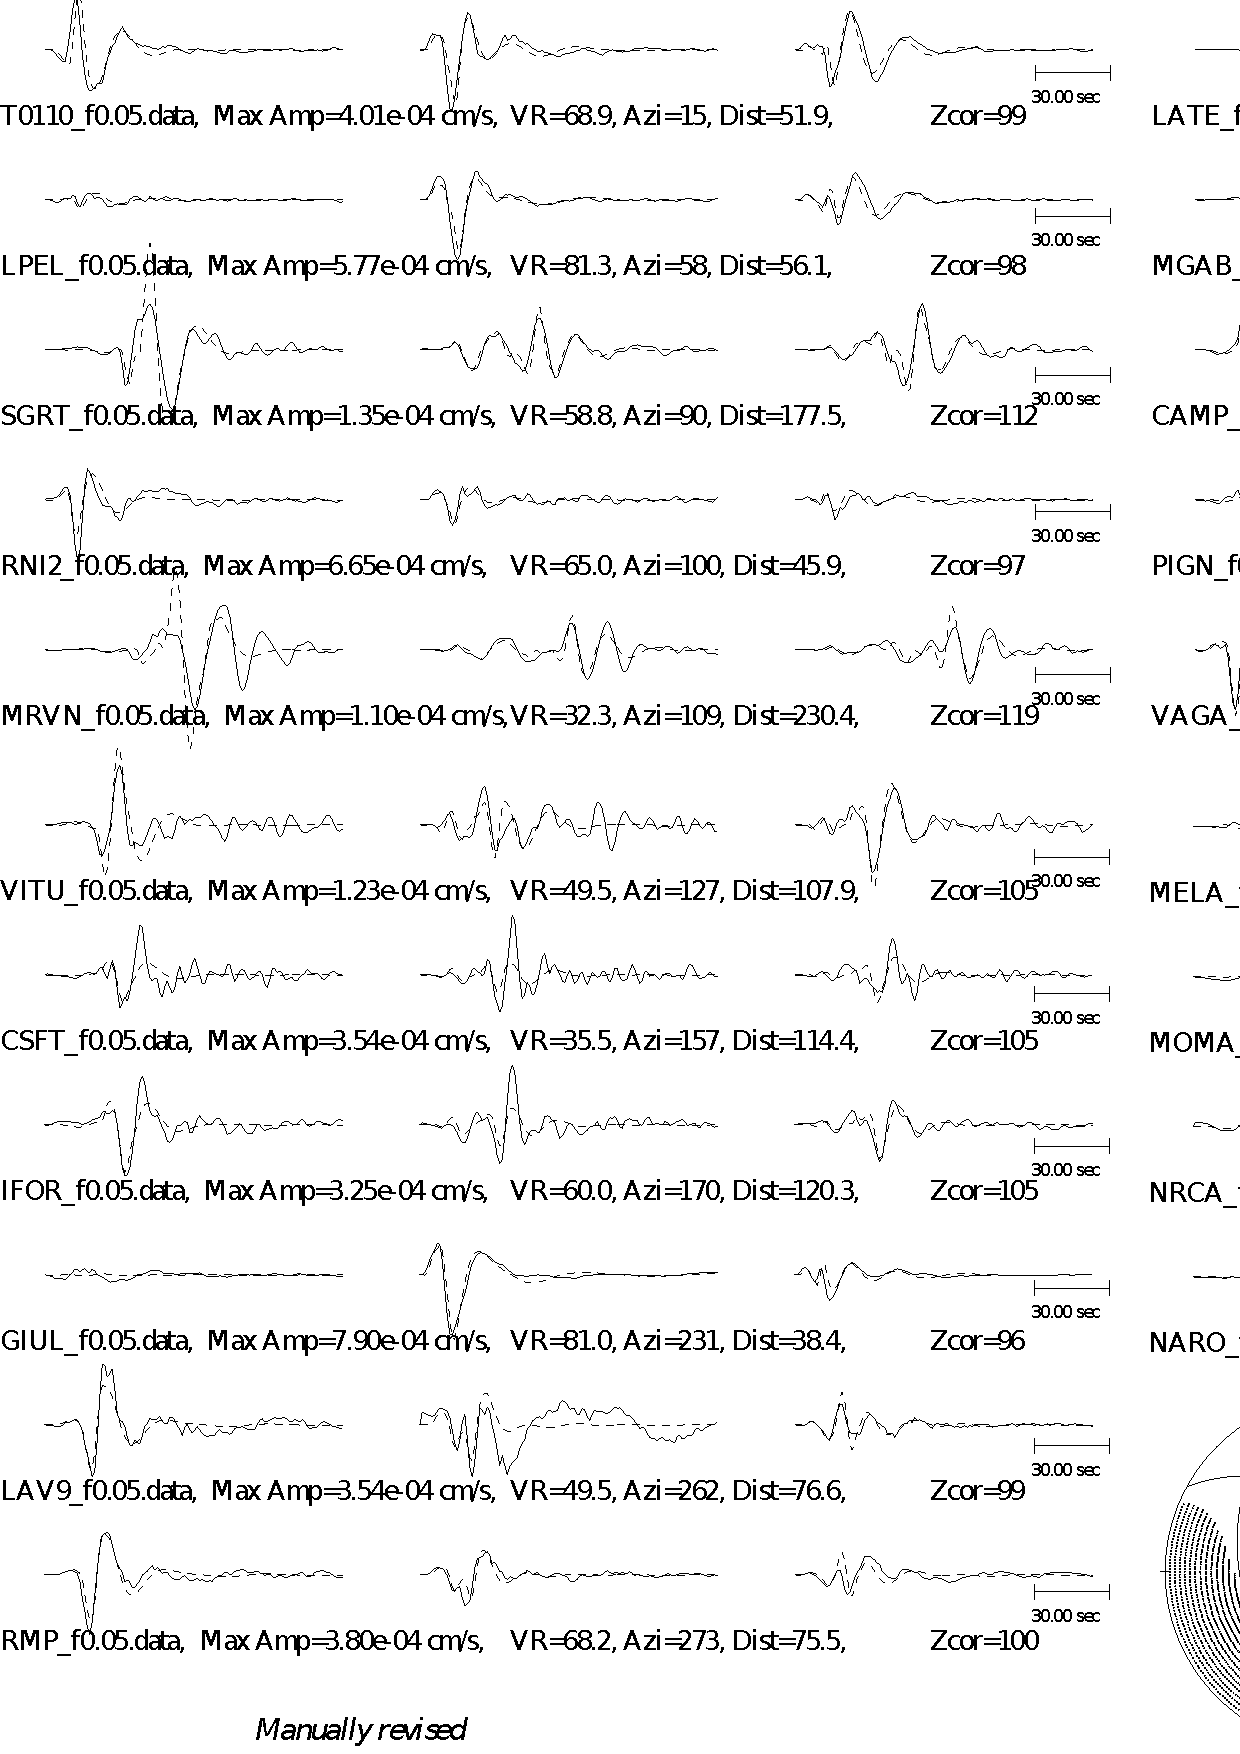
\includegraphics[width=1\linewidth]{S2_Focal_synthetics}
\caption{Estimated focal mechanism and comparison of observed (solid lines) and estimated synthetic seismograms (dashed lines) for the Mw 4.4 mainshock. The three components at 22 receiver locations are shown. This figure is a modified version from the original one provided by the INGV \url{http://webservices.ingv.it/webservices/ingv_ws_map/data/tdmt/15111/73711301_86_tdmt_reviewer_solution.pdf}.}
\label{fig:S2_focal_mechanism}
\end{figure}
\Assignment{Hugo} \WorkInProgressRevTask
\end{Answer}
%
%



\begin{ReviewerComment}{1}
\noindent 
L104. "According to a geological study of the location of the main event and its focal mechanism (Supplementary Material Table S1), this event ruptured the Liri fault (Roberts and Michetti, 2004), which is one of the major active normal faults mapped in this region." \\

I did not see the evidence for choosing one of the two fault implied from the focal mechanism. (I looked in the supplement.) This is a critical piece, since the assumed fault plane is referenced in Figure 5.
\end{ReviewerComment}


\begin{Answer}
Thnaks for your comment. We think that the evidence can be observed looking at the surface geololy. According to the work from \cite{Falcucci2016active} \\
\hfill === Read paper and then we discuss \\ 
\hfill ===  Modify the text (citation) Hugo \\
\hfill ===  Modify figure accordingly  David\\
In order to emphasize the superficial scarps, in the revised version we improve the former figure 1, increasing the resolution of the topography. We hope that this evidence is clearer in this version of the manuscript.
\Assignment{Hugo} \WorkInProgressRevTask
\end{Answer}
%
%



\begin{ReviewerComment}{1}
\noindent 
From one event, it is difficult to understand the significance of the findings. Did the authors point their same set of tools at a couple other events? What if all mainshocks in this region have foreshock sequences? What is the meaning of "normal" seismicity sequences in this region? In other words, is this one earthquake significant, or do many other earthquakes -- when examined this closely -- show such complexity? In particular, are there foreshock sequences such as Cluster 1?

\end{ReviewerComment}


\begin{Answer}
\hfill PIERO WILL ANSWER THIS
\Assignment{Hugo} \WorkInProgressRevTask
\end{Answer}
%
%



\begin{ReviewerComment}{1}
\noindent 
I have never done Coulomb stress modeling, but it seems like it was developed for this kind of study, where the fault is (likely) known, and the mechanism would predict aftershock occurrences in certain regions.
\end{ReviewerComment}


\begin{Answer}
We totally agree with reviewer \# 1 about the potential of performing a Coulomb stress analysis in the region. However, the geometry of the faults that were activated during this sequence are not known (except from the one associated to the mainshock). In addition, the focal mechanisms of most of the earthquakes in the sequence can not be determined due to their small size, noise levels and limitted azimuthal coverage. Therefore, the available information does not allow to perform any Coulomb stress analysis of this sequence.
\Assignment{Hugo} \WorkInProgressRevTask
\end{Answer}
%
%



\begin{ReviewerComment}{1}
\noindent 
Figure 5 is key and needs improvements. There's too much white space to see the details.  Perhaps zoom into +/- 1 km and then leave the full +/- 3 km version in the supplement? No legend is needed, since the caption will tell us that a=Cluster1, b=Cluster2, etc. Save space by not displaying a, b, three times.

\end{ReviewerComment}


\begin{Answer}
\Assignment{Hugo} \WorkInProgressRevTask
\end{Answer}
%
%


\begin{ReviewerComment}{1}
\noindent 
Figure 5a. Perhaps a dashed line for the assumed auxiliary plane? It is not clearcut to me that the dots are collapsing to a plane. (See also point about fault plane vs auxiliary plane above.)

\end{ReviewerComment}


\begin{Answer}
\Assignment{Hugo} \WorkInProgressRevTask
\end{Answer}
%
%


\begin{ReviewerComment}{1}
\noindent 
If the choice of fault plane is in question, then it would be good to see an alternative version of Figure 5, where the projection planes are chosen based on the now-assumed auxiliary plane (under the assumption that it is the mainshock fault plane).

\end{ReviewerComment}


\begin{Answer}
\Assignment{Hugo} \WorkInProgressRevTask
\end{Answer}
%
%


\begin{ReviewerComment}{1}
\noindent 
Most of the results imply complexity associated with the aftershock patterns. Is this exceptional? Are we to assume that the mainshock was complicated and that the aftershocks illuminate the region? Or that these adjacent faults were triggered by the mainshock?

\end{ReviewerComment}


\begin{Answer}
\Assignment{Hugo} \WorkInProgressRevTask
\end{Answer}
%
%




\begin{ReviewerComment}{1}
\noindent 
Fig. 2: mention diurnal variability in the white curve. Probably 6pm-6am or 18:00-06:00 is a better label. I don't think any legend is needed in b and c.

\end{ReviewerComment}


\begin{Answer}
\Assignment{Hugo} \WorkInProgressRevTask
\end{Answer}
%
%


\begin{ReviewerComment}{1}
\noindent 
Figure 4. t=0 needs to be a tick mark, since that's the mainshock. (That way, you do not need the legend item for the mainshock either.)

\end{ReviewerComment}


\begin{Answer}
\Assignment{Hugo} \WorkInProgressRevTask
\end{Answer}
%
%


\begin{ReviewerComment}{1}
\noindent 
Figure 4. I'm not finding the 90\% line to be helpful or representative of the distributions. Is it needed?

\end{ReviewerComment}


\begin{Answer}
\Assignment{Hugo} \WorkInProgressRevTask
\end{Answer}
%
%

\section*{Reviewer \#2}


\subsection*{Summary}

This is an overall strong paper that is suitable for publication following minor edits. The authors perform a detailed analysis of foreshocks and aftershocks of the Mw 4.4 2019 Balsorano earthquake and demonstrate the complexity of these sequences, including apparent initiation on an antithetic fault. The authors first enhance the existing earthquake catalog using template matching. Next, they cluster events based on waveform similarity. Last, they relocate the majority of the newly detected events using the double-difference algorithm. The paper is clearly organized and the implications related to initiation processes and rupture complexities are very interesting.  \\


\subsection*{Template matching}

\begin{ReviewerComment}{1}
\noindent 
Enhancing the catalog to 714 events is a significant improvement. However, using 23 out of 135 available catalog events as template earthquakes seems low and may prevent additional event detection. Is the 1-second pre-pick discussed on line 132 before the P-phase arrival? If so, why is the pre-pick time so long? This introduces noise to the signal - about 25% of the waveform - that decreases the signal-to-noise ratio that is then used in template selection. More templates would likely meet the SNR criteria with a shorter pre-pick, unless I misunderstand this 1-second pre-pick.

\end{ReviewerComment}


\begin{Answer}
\Assignment{Hugo} \WorkInProgressRevTask
\end{Answer}
%
%



\begin{ReviewerComment}{1}
\noindent 
It would be helpful to provide the hypocentral locations and magnitudes of template events in Table S4, and include a map of template earthquakes to give a better idea whether detections (including the 13-15 km depth concentration of seismicity) are biased by template locations. Further, focal mechanisms of templates if available would provide additional information about potential biases in earthquake detection (i.e., if locations and focal mechanisms of templates are very similar, dissimilar events will not be detected). That being said, the results do not seem to be over-interpreted and a discussion of these potential biases would be adequate.

\end{ReviewerComment}


\begin{Answer}
\Assignment{Hugo} \WorkInProgressRevTask
\end{Answer}
%
%



\begin{ReviewerComment}{1}
\noindent 
The method to determine the magnitude of earthquakes detected with template matching makes sense. However, the least-square fitting to obtain a linear model for magnitudes using only 23 earthquakes is unlikely to be robust. I suggest using more earthquakes in the INGV catalog to develop this model prior to applying it to the newly detected events.

\end{ReviewerComment}


\begin{Answer}
\Assignment{Hugo} \WorkInProgressRevTask
\end{Answer}
%
%

\subsection*{Clustering}

\begin{ReviewerComment}{1}
\noindent 
Line 169 states that members of the same cluster should share similarities in position and rupture mechanism.  However, the locations in cluster 3 vary widely. The station nearest to the study region will not have large S-P time differences for most of the events; therefore, events in different locations with similar mechanisms might appear similar. Please expand on this in the waveform-based clustering section of methods, or consider using a farther station (or combining the results of multiple stations) for the waveform-based clustering.

\end{ReviewerComment}


\begin{Answer}
\Assignment{Hugo} \WorkInProgressRevTask
\end{Answer}
%
%



\begin{ReviewerComment}{1}
\noindent 
The stacked waveform for cluster 3 in Figure 3c is smaller amplitude than the other stacked waveforms and it is difficult to identify phase arrivals. This is likely because events in this cluster are not as similar as other clusters. Please discuss the similarity in this cluster more in the main text.

\end{ReviewerComment}


\begin{Answer}
\Assignment{Hugo} \WorkInProgressRevTask
\end{Answer}
%
%


\subsection*{Aseismic slip}


\begin{ReviewerComment}{1}
\noindent 
Pre-seismic: Line 302 in the Conclusion states that there is a lack of repeating earthquakes in the foreshock sequence. This should be mentioned earlier, perhaps near Lines 256-261 in the Results and Discussion section where the lack of evidence for aseismic slip is discussed.

\end{ReviewerComment}


\begin{Answer}
\Assignment{Hugo} \WorkInProgressRevTask
\end{Answer}
%
%



\begin{ReviewerComment}{1}
\noindent 
Post-seismic: Line 275 attributes clusters 4 and 5 to afterslip on the main fault. Afterslip can also trigger seismicity/aftershocks off of the main fault (Inbal et al., 2017) but this is still a reasonable mechanism. Is there a log(time) dependence in spatial expansion in these clusters that may also indicate aseismic slip? Are any repeating earthquakes present in the aftershock sequence that may be indicative of co-planar afterslip? I assume not since the foreshocks are the most highly correlated, but it is still worth mentioning in the discussion of afterslip as a mechanism.
\end{ReviewerComment}


\begin{Answer}
\begin{figure}[!h]
\begin{center}
 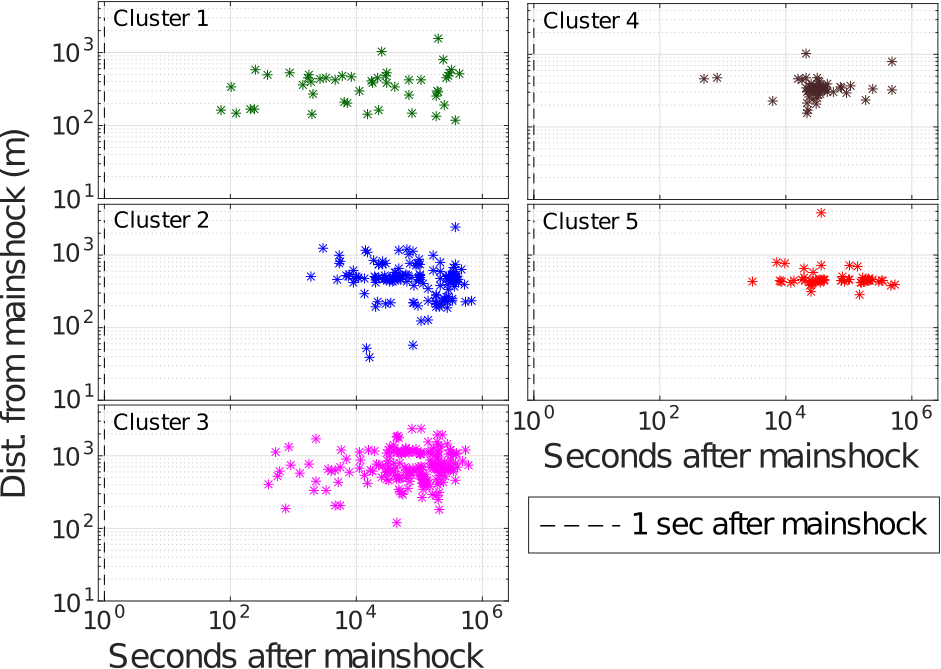
\includegraphics[width=0.8\linewidth]{S3_loglog_time.png} 
\end{center}
\end{figure}
\Assignment{Hugo} \WorkInProgressRevTask
\end{Answer}
%
%




\begin{ReviewerComment}{1}
\noindent 
Be consistent with defining small and medium (or moderate-sized) earthquakes. Line 24 has small earthquakes classified as  Mw<5, Line 54 has medium-events listed as Mw < 6, and Line 83 has small-magnitude events classified as Mw<6. It is most common to consider M 4-6 as moderate-sized and Mw < 3 as small magnitude earthquakes. I recommend grouping small to moderate-sized earthquakes as Mw < 6 consistently.

\end{ReviewerComment}


\begin{Answer}
\Assignment{Hugo} \WorkInProgressRevTask
\end{Answer}
%
%




\begin{ReviewerComment}{1}
\noindent 
Figure 1: The topography in this figure is poor resolution. Is better resolution topography data available? If not, it may be better to remove it because it is distracting and does not add much to the figure. I also recommend adding mapped faults - including the Liri fault. Add scale bar to the main map.

\end{ReviewerComment}


\begin{Answer}
\Assignment{Hugo} \WorkInProgressRevTask
\end{Answer}
%
%



\begin{ReviewerComment}{1}
\noindent 
Figure 3: It is difficult to differentiate aftershock clusters on (3b); expand the time series so temporal patterns are visible. Alternatively, you can plot cumulative events per cluster rather than combining them together.  

\end{ReviewerComment}


\begin{Answer}
\Assignment{Hugo} \WorkInProgressRevTask
\end{Answer}
%
%



\begin{ReviewerComment}{1}
\noindent 
Supplementary Figure S1: The distance threshold is listed here as 5.3 but is given as 5.5 in the main text (line 166). Please fix this. Change "form dendrogram" to "FROM dendrogram"

\end{ReviewerComment}


\begin{Answer}
\Assignment{Hugo} \WorkInProgressRevTask
\end{Answer}
%
%



\begin{ReviewerComment}{1}
\noindent 
Supplementary Figure S2 is not discussed in the main text. Based on the figure and figure caption alone, the purpose of this figure is not clear. Either add in a reference to it in the main text, or consider removing it.

\end{ReviewerComment}


\begin{Answer}
\Assignment{Hugo} \WorkInProgressRevTask
\end{Answer}
%
%


minor edits

\begin{ReviewerComment}{1}
\noindent 
*        Lines 37-38: "…each cluster in this sequence has a distinct triggering mechanism." In the Conclusion clusters 2\&3 and 4\&5 are grouped together in terms of triggering mechanisms; therefore, each cluster does not have a distinct mechanism.  

\end{ReviewerComment}


\begin{Answer}
\Assignment{Hugo} \WorkInProgressRevTask
\end{Answer}
%
%



\begin{ReviewerComment}{1}
\noindent 

\end{ReviewerComment}


\begin{Answer}
\Assignment{Hugo} \WorkInProgressRevTask
\end{Answer}
%
%



\begin{ReviewerComment}{1}
\noindent 

\end{ReviewerComment}


\begin{Answer}
\Assignment{Hugo} \WorkInProgressRevTask
\end{Answer}
%
%



\begin{ReviewerComment}{1}
\noindent 

\end{ReviewerComment}


\begin{Answer}
\Assignment{Hugo} \WorkInProgressRevTask
\end{Answer}
%
%



\begin{ReviewerComment}{1}
\noindent 

\end{ReviewerComment}


\begin{Answer}
\Assignment{Hugo} \WorkInProgressRevTask
\end{Answer}
%
%



\begin{ReviewerComment}{1}
\noindent 

\end{ReviewerComment}


\begin{Answer}
\Assignment{Hugo} \WorkInProgressRevTask
\end{Answer}
%
%







Specific comments:





Minor edits (suggested additions are in all caps):


*        Line 40 - I suggest changing "incoming" to another term that expresses more of an expectation in time, such as upcoming, imminent, impending, or forthcoming.  
*        Line 41 - "behind the triggering AND NUCLEATION of earthquakes"
*        Lines 40-41: This introductory sentence would be more compelling if you add in the importance of precursory signals beyond models. Yes, models are important, but they are important because characterizing earthquakes is important.
*        Line 47 - What is meant by "more significant?" Most compelling? Most impactful?
*        Line 54 -  change "even for" to "PARTICULARLY for MORE frequent" to emphasize that small to moderate-sized %events occur more frequently than larger events and are %therefore useful to study.
*        Line 55 - "Improved observations MAY shed light on the physical processes that occur during the triggering AND NUCLEATION of earthquakes…"
*        Line 73 - "ASEISMIC slip processes"
*        Line 85 - Remove "last" before "more recent studies "
*        Line 101 - Change "~15 km" to the actual hypocenter depth of 14 km
*        "Poli et al., 2020b" - Fix citation throughout



\bibliography{../bibliography}
\bibliographystyle{apalike}


\end{document}










